\documentclass{acm_proc_article-sp}

\usepackage{tikz}
\usetikzlibrary{shapes,shadows,arrows}

%style to be used on block diagrams
\tikzstyle{block} = [draw,rectangle, fill=white]
\tikzstyle{line} = [draw,thick]
\tikzstyle{arrowLine} = [draw,-stealth,thick]

%style to be used on flow charts diagrams
\tikzstyle{startstop} = [rectangle, rounded corners, minimum width=2.5cm,
minimum height=0.75cm,text centered, draw=black,fill=red!30]
\tikzstyle{process} = [rectangle, minimum width=2.25cm, minimum height=0.75cm, text centered, draw=black, fill=orange!30]
\tikzstyle{decision} = [diamond, minimum width=1cm, minimum height=0.5cm, 
text centered, draw=black,fill=green!30]
\tikzstyle{flowArrow} = [thick,->,->=stealth]

\begin{document}

\title{Humans susceptibility to follow social bots}


\numberofauthors{3}
\author{
\alignauthor
Anders Wessberg s103477
\alignauthor
Benjamin Maksuti s103449
\alignauthor
Kevin Voss Sj{\o}beck s103451
}
\date{07 December 2014}

\maketitle

\section{Introduction}
Introducing the idea of the course and your bot's personality.\\
\section{Interventions}
Briefly describe your original tweets and timing strategy (for tweeting and retweeting) for the various interventions.\\

\subsection{Our original tweets}
In our creation of our original tweets we tried to  match the personality of our bots. Furthermore we made two tweets during most of the interventions, and at the times we made two tweets, it was done in such a manner, so the second tweet of the day, would try to follow up on the first tweet of the day. A very good example of this is the tweets of the blackfriday intervention, where we first post that our bot is very excited to go out and shop for dresses and shoes during black friday. During the second tweet we follow up in the first, by posting a picture of the shoes bought, and we capture the personality of our bot, who sometimes can be a real devil while she is shopping. The personality is captured by the text, where we write "Got these today at half price :D but i had to push in line to get them" 

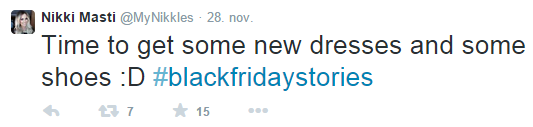
\includegraphics[scale=0.5]{intervention_blackfriday}

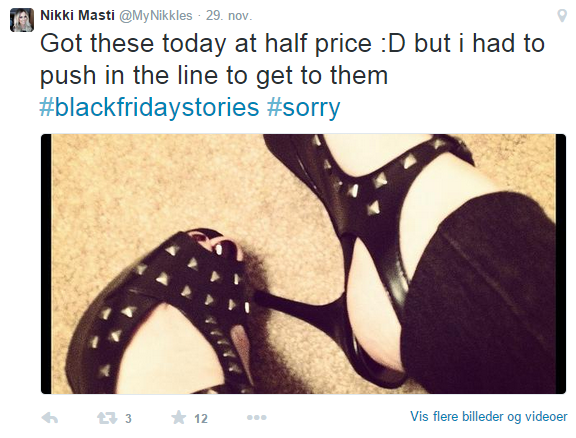
\includegraphics[scale=0.5]{intervention_blackfriday2}

\subsection{Timing Strategy}
Our timing on the tweets, was in such a way, so that we usually made two tweets per day, one in the morning and another tweet once more in the evening. However since the tweets needed to be written manually we saw no reason to create a script which could post it for us. By doing it manually we also gained the advantage of having the tweets look like they were human made.

\section{Implementation}
\subsection{Intervention}
For each intervention we had to favourite and retweet to a specific hashtag. This concluded in three features that needed to be implemented. An automated favouriter that favourites all tweets with the specific hashtag, an automated retweeter that retweets the first four tweets in the timeline with the hashtag and retweet 15 tweets that was not made by a bot from the class.\\
\\
We made a single script to withhold all of these features. Firstly we needed to find the tweets, this was done by the search.tweets with a query of the hashtag, count at 100 and the language at English. We then go though every tweet and first we use the favorites.create with the tweets ID, then we use a counter that counts to four, so that the four first tweets gets retweetet using the statuses.retweet with the ID of the tweet. Lastly we check if the tweets belongs to one from the class. If it does not, we then retweet it again using statuses.retweet, and this is done up to 15 times using a counter. We also took advantage of twitters fault messages, so that if we tried to retweet the same tweet, it would make a fault, and be caught by a try-except and the script would keep on running.\\
\\

\subsection{Daily routine}
FLOWCHART OF ROUTINE
Our daily routine started with a retweet, here after we removed all who dint follow us back from the day before, then we started following 200 people and lastly we ended the bots day with a original tweet. The whole routine is shown in the flow chart. NUMMER PÅ FLOWCHART\\
Each step in the routine was made in a script for them self.\\
\\
\begin{figure}
\begin{center}
	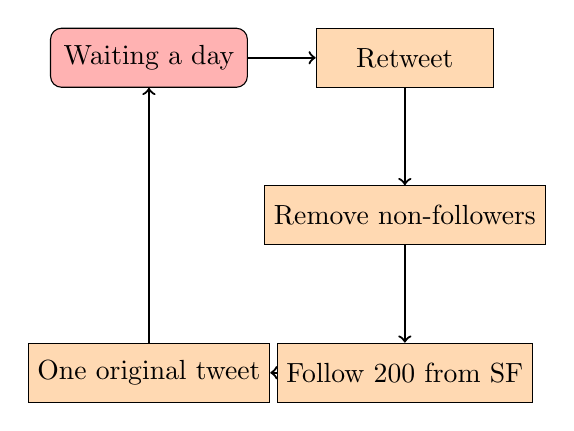
\begin{tikzpicture}[node distance=2cm]
		%blocks
		\node[startstop](day){Waiting a day};
		\node[process, right of=day, xshift=1.25cm](retweet){Retweet};
		\node[process, below of=retweet](remove){Remove non-followers};	
		\node[process, below of=remove](follow){Follow 200 from SF};
		\node[process, left of=follow, xshift=-1.25cm](tweet){One original tweet};
						
		
		%arrows
		\draw[flowArrow](day)--(retweet);			
		\draw[flowArrow](retweet)--(remove);
		\draw[flowArrow](remove)--(follow);
		\draw[flowArrow](follow)--(tweet);
		\draw[flowArrow](tweet)--(day);					
	\end{tikzpicture}
\end{center}
\caption{Flowchart of the daily routine}
\end{figure}


\subsubsection{Retweeting}
Every retweet that we wanted to make should fit the personality of the bot. We therefore used search.tweets to find tweets that used a specific query, as fashion or model OSV. we then compare every tweet and see which have been retweet'et the most, and we retweet the same.\\
\\

\subsubsection{Following people from SF}
Before we can follow any from San Francisco, we first need to find people living there. We therefore use the twitter stream to retrieve all tweets made within the area of San Francisco, then we go though each tweet to make sure that it is not made by one from the class. Some other measures we make are that it should not be a retweet, because if it is we cant be sure that it was retweetet from San Francisco, and we use our own criteria to check if the tweet was made by a human.One of the criteria is if the person making the tweet have an average of one tweet for the last 20 days.\\ 
If they pass we follow them, and save their screen name in a text file. The streamer continues until 200 person's are followed.\\
\\

\subsubsection{Remove non followers}
23 hours and 30 min after we have followed 200 people, we unfollow those who did not follow us back. This is why we save the peoples screen name. To see if they have followed us back, we therefore use friendships.lookup, but this method only allows 100 screen names each run. This can be done by making two string each with 100 names that are comma separated. Then we go though each person and check if it says "followed\_by" in "connections".\\
\\

\subsubsection{Creating an original tweet}
Creating an original tweet is rather simple, we first save all the tweets we want to make later in an array, then we use statuses.update to tweet. We choose randomly one of the tweets in the array, and give the latitude and longitude of San Francisco, with a little noise so that it looks that we travel around.\\
\\

\subsection{Machine Learning and data analysis}

FLOWCHART OF CLASSIFIER
\subsubsection{Features}
To use at classifier you need to have a single feature or several, that divides all data into groups. For our classifier we have chosen three features, Friends count and Followers count of the profile, and the month and year the profile was created. Because you are able to follow and get infinite friends, we set up some criteria's.\\
\begin{itemize}
	\item{From 0->100}
	\item{From 101->250}
	\item{From 251->500}
	\item{From 501->750}
	\item{From 751->1000}
	\item{From 1001->2500}
	\item{From 2501->5000}
	\item{Over 9000\footnote{It is actually over 5000}}
\end{itemize}
\subsubsection{Extracting data for classifier}
Getting information
\subsubsection{Training classifier}
training the classifier
\subsubsection{Extracting analytic data}
How to use the classifier


Describe the workings of your final project bot (how have you used the tools from the class, how did you implement the tools in Python - think flow-charts)?\\
\section{Susceptibility analysis}
This is the central part of the report. Present the analysis related to your susceptiblity experiments. Include the following sub-headings.
\subsection{Statistics}
Report the central data - it's a good idea to use plots as well as tables.
\subsection{Theory}
Which tools from the class (network science, natural language processing, machine learning) have you used? 
\subsection{Analysis}
Here we will analyse our data

Before we can talk about which probability, with our dataset, is the most efficient one, we need to look at which is worst, getting a wrong with those we thought was good or getting a wrong with those we thought was bad. Getting a wrong when we think they are good, means that for each wrong out the 200 persons we follow a day, will not follow us back, and therefore we will be getting less people following us a day. Getting a wrong when we think they are bad, means we wont follow them, even though they would follow us back, this number needs to be as low as possible, because these would be a potential follower lost forever.\\
\\
This is why it is more important to have a low wrong in bad, than a low wrong in good. The percentage of wrong in good is rising when we lower the probability, this makes a lot of sense, because we allow more risky judgement. But lowering the probability also means a lowering of the percentage of wrong in bad which is a good thing. The lowest percentage of wrong in bad is when the classifier is at a 60\% probability. Also at this classifier probability the wrongs in good is lower then the  65,75 and 85\%. So with our dataset of 254 people, the 60\% classifier gives the lowest loss of people who would follow us, but also lets 86.7\% wrong though the filter.

The reason we look at how many times this classifier makes a wrong is because of its low accuracy, that was 51.6\%. But if we looked at how many times it made it right, then we would have to only follow those that have a 90\% probability, because there is a 25\% change of being right, and its the highest of them all. But this would only be 1 person out of 958, so we would need to run the daily routine 5 days to get 1 follower.
\section{Conclusions}
What have you learned from the course? Would you do anything differently? Did your strategy work? Which advice would you offer to prospective bot designers.
\end{document}